The figure shows equipotential lines (orange) in a region of space, in equal steps of \SI{2}{\V}.

\begin{center}
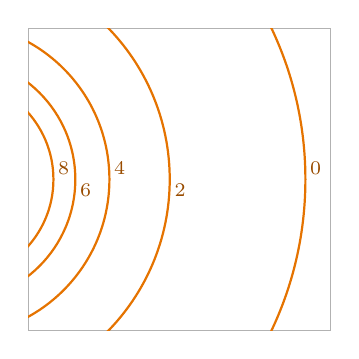
\begin{tikzpicture}
 \draw[black!30] (0.00,-1.92) rectangle (3.84,1.92);
 \begin{scope}
 \clip (0.00,-1.92) rectangle (3.84,1.92);
 \draw[orange!90!black, thick] (-0.96,0.00) circle (1.280);
 \draw[orange!90!black, thick] (-0.96,0.00) circle (1.558);
 \draw[orange!90!black, thick] (-0.96,0.00) circle (1.991);
 \draw[orange!90!black, thick] (-0.96,0.00) circle (2.757);
 \draw[orange!90!black, thick] (-0.96,0.00) circle (4.480);
 \end{scope}
 \node[above right, inner sep=1.5pt, text=orange!60!black] at (0.32,0) {\scriptsize \SI{8}{\V}};
 \node[below right, inner sep=1.5pt, text=orange!60!black] at (0.60,0) {\scriptsize \SI{6}{\V}};
 \node[above right, inner sep=1.5pt, text=orange!60!black] at (1.03,0) {\scriptsize \SI{4}{\V}};
 \node[below right, inner sep=1.5pt, text=orange!60!black] at (1.80,0) {\scriptsize \SI{2}{\V}};
 \node[above right, inner sep=1.5pt, text=orange!60!black] at (3.52,0) {\scriptsize \SI{0}{\V}};
\end{tikzpicture}
\end{center}

\begin{abcliste}
\abc Copy the figure and draw some field lines, with arrows.
\abc Mark the region where the field is strongest. Give a reason.
\abc Three students drew the field lines (blue) as in the diagrams (1) to (3). What is wrong with each of them?
\end{abcliste}

\begin{center}
\begin{tikzpicture}
 \draw[black!30] (0.00,-1.92) rectangle (3.84,1.92);
 \begin{scope}
 \clip (0.00,-1.92) rectangle (3.84,1.92);
 \draw[orange!90!black, thick] (-0.96,0.00) circle (1.280);
 \draw[orange!90!black, thick] (-0.96,0.00) circle (1.558);
 \draw[orange!90!black, thick] (-0.96,0.00) circle (1.991);
 \draw[orange!90!black, thick] (-0.96,0.00) circle (2.757);
 \draw[orange!90!black, thick] (-0.96,0.00) circle (4.480);
\draw[blue!75!black, thick] plot[smooth] coordinates {(3.32,-4.76) (-0.42,-0.59)};
\draw[blue!75!black, thick, -{Stealth[length=1.7mm, width=1.4mm]}] (2.766,-4.142) -- (2.699,-4.067);
\draw[blue!75!black, thick] plot[smooth] coordinates {(4.47,-3.39) (-0.28,-0.42)};
\draw[blue!75!black, thick, -{Stealth[length=1.7mm, width=1.4mm]}] (3.766,-2.950) -- (3.681,-2.897);
\draw[blue!75!black, thick] plot[smooth] coordinates {(5.19,-1.76) (-0.19,-0.22)};
\draw[blue!75!black, thick, -{Stealth[length=1.7mm, width=1.4mm]}] (4.393,-1.532) -- (4.297,-1.504);
\draw[blue!75!black, thick] plot[smooth] coordinates {(5.19,1.76) (-0.19,0.22)};
\draw[blue!75!black, thick, -{Stealth[length=1.7mm, width=1.4mm]}] (4.393,1.532) -- (4.297,1.504);
\draw[blue!75!black, thick] plot[smooth] coordinates {(4.47,3.39) (-0.28,0.42)};
\draw[blue!75!black, thick, -{Stealth[length=1.7mm, width=1.4mm]}] (3.766,2.950) -- (3.681,2.897);
\draw[blue!75!black, thick] plot[smooth] coordinates {(3.32,4.76) (-0.42,0.59)};
\draw[blue!75!black, thick, -{Stealth[length=1.7mm, width=1.4mm]}] (2.766,4.142) -- (2.699,4.067);
 \end{scope}
 \node[above right, inner sep=1.5pt, text=orange!60!black] at (0.32,0) {\scriptsize \SI{8}{\V}};
 \node[below right, inner sep=1.5pt, text=orange!60!black] at (0.60,0) {\scriptsize \SI{6}{\V}};
 \node[above right, inner sep=1.5pt, text=orange!60!black] at (1.03,0) {\scriptsize \SI{4}{\V}};
 \node[below right, inner sep=1.5pt, text=orange!60!black] at (1.80,0) {\scriptsize \SI{2}{\V}};
 \node[above right, inner sep=1.5pt, text=orange!60!black] at (3.52,0) {\scriptsize \SI{0}{\V}};
 \node[below] at (1.92,-1.97) {(1)};
\end{tikzpicture}
\quad
\begin{tikzpicture}
 \draw[black!30] (0.00,-1.92) rectangle (3.84,1.92);
 \begin{scope}
 \clip (0.00,-1.92) rectangle (3.84,1.92);
 \draw[orange!90!black, thick] (-0.96,0.00) circle (1.280);
 \draw[orange!90!black, thick] (-0.96,0.00) circle (1.558);
 \draw[orange!90!black, thick] (-0.96,0.00) circle (1.991);
 \draw[orange!90!black, thick] (-0.96,0.00) circle (2.757);
 \draw[orange!90!black, thick] (-0.96,0.00) circle (4.480);
\draw[blue!75!black, thick] plot[smooth] coordinates {(-0.96,-1.42) (-0.47,-1.34) (-0.04,-1.09) (0.27,-0.71) (0.44,-0.25) (0.44,0.25) (0.27,0.71) (-0.04,1.09) (-0.47,1.34) (-0.96,1.42)};
\draw[blue!75!black, thick, -{Stealth[length=1.7mm, width=1.4mm]}] (0.440,-0.050) -- (0.440,0.050);
\draw[blue!75!black, thick] plot[smooth] coordinates {(-0.96,-1.76) (-0.36,-1.65) (0.17,-1.35) (0.56,-0.88) (0.77,-0.31) (0.77,0.31) (0.56,0.88) (0.17,1.35) (-0.36,1.65) (-0.96,1.76)};
\draw[blue!75!black, thick, -{Stealth[length=1.7mm, width=1.4mm]}] (0.770,-0.050) -- (0.770,0.050);
\draw[blue!75!black, thick] plot[smooth] coordinates {(-0.96,-2.36) (-0.15,-2.22) (0.56,-1.81) (1.08,-1.18) (1.36,-0.41) (1.36,0.41) (1.08,1.18) (0.56,1.81) (-0.15,2.22) (-0.96,2.36)};
\draw[blue!75!black, thick, -{Stealth[length=1.7mm, width=1.4mm]}] (1.360,-0.050) -- (1.360,0.050);
\draw[blue!75!black, thick] plot[smooth] coordinates {(-0.96,-3.60) (0.27,-3.38) (1.35,-2.76) (2.16,-1.80) (2.59,-0.63) (2.59,0.63) (2.16,1.80) (1.35,2.76) (0.27,3.38) (-0.96,3.60)};
\draw[blue!75!black, thick, -{Stealth[length=1.7mm, width=1.4mm]}] (2.590,-0.050) -- (2.590,0.050);
 \end{scope}
 \node[above right, inner sep=1.5pt, text=orange!60!black] at (0.32,0) {\scriptsize \SI{8}{\V}};
 \node[below right, inner sep=1.5pt, text=orange!60!black] at (0.60,0) {\scriptsize \SI{6}{\V}};
 \node[above right, inner sep=1.5pt, text=orange!60!black] at (1.03,0) {\scriptsize \SI{4}{\V}};
 \node[below right, inner sep=1.5pt, text=orange!60!black] at (1.80,0) {\scriptsize \SI{2}{\V}};
 \node[above right, inner sep=1.5pt, text=orange!60!black] at (3.52,0) {\scriptsize \SI{0}{\V}};
 \node[below] at (1.92,-1.97) {(2)};
\end{tikzpicture}
\quad
\begin{tikzpicture}
 \draw[black!30] (0.00,-1.92) rectangle (3.84,1.92);
 \begin{scope}
 \clip (0.00,-1.92) rectangle (3.84,1.92);
 \draw[orange!90!black, thick] (-0.96,0.00) circle (1.280);
 \draw[orange!90!black, thick] (-0.96,0.00) circle (1.558);
 \draw[orange!90!black, thick] (-0.96,0.00) circle (1.991);
 \draw[orange!90!black, thick] (-0.96,0.00) circle (2.757);
 \draw[orange!90!black, thick] (-0.96,0.00) circle (4.480);
\draw[blue!75!black, thick] plot[smooth] coordinates {(-0.40,-1.60) (4.40,-1.60)};
\draw[blue!75!black, thick, -{Stealth[length=1.7mm, width=1.4mm]}] (0.430,-1.600) -- (0.530,-1.600);
\draw[blue!75!black, thick] plot[smooth] coordinates {(-0.40,-1.12) (4.40,-1.12)};
\draw[blue!75!black, thick, -{Stealth[length=1.7mm, width=1.4mm]}] (0.430,-1.120) -- (0.530,-1.120);
\draw[blue!75!black, thick] plot[smooth] coordinates {(-0.40,-0.64) (4.40,-0.64)};
\draw[blue!75!black, thick, -{Stealth[length=1.7mm, width=1.4mm]}] (0.430,-0.640) -- (0.530,-0.640);
\draw[blue!75!black, thick] plot[smooth] coordinates {(-0.40,0.64) (4.40,0.64)};
\draw[blue!75!black, thick, -{Stealth[length=1.7mm, width=1.4mm]}] (0.430,0.640) -- (0.530,0.640);
\draw[blue!75!black, thick] plot[smooth] coordinates {(-0.40,1.12) (4.40,1.12)};
\draw[blue!75!black, thick, -{Stealth[length=1.7mm, width=1.4mm]}] (0.430,1.120) -- (0.530,1.120);
\draw[blue!75!black, thick] plot[smooth] coordinates {(-0.40,1.60) (4.40,1.60)};
\draw[blue!75!black, thick, -{Stealth[length=1.7mm, width=1.4mm]}] (0.430,1.600) -- (0.530,1.600);
 \end{scope}
 \node[above right, inner sep=1.5pt, text=orange!60!black] at (0.32,0) {\scriptsize \SI{8}{\V}};
 \node[below right, inner sep=1.5pt, text=orange!60!black] at (0.60,0) {\scriptsize \SI{6}{\V}};
 \node[above right, inner sep=1.5pt, text=orange!60!black] at (1.03,0) {\scriptsize \SI{4}{\V}};
 \node[below right, inner sep=1.5pt, text=orange!60!black] at (1.80,0) {\scriptsize \SI{2}{\V}};
 \node[above right, inner sep=1.5pt, text=orange!60!black] at (3.52,0) {\scriptsize \SI{0}{\V}};
 \node[below] at (1.92,-1.97) {(3)};
\end{tikzpicture}
\end{center}
